% -*- root: ../../main.tex -*-
%!TEX root = ../../main.tex
% this file is called up by main.tex
% content in this file will be fed into the main document
% vim:textwidth=80 fo=cqt

As  evidenced by  the  results of  the constant  current  charge, discharge  and
dynamic  simulation runs,  the basic  \gls{spm} suffers  from a  \emph{critical}
drawback. The lack of electrolyte dynamics in the conventional \gls{spm} results
in poor  voltage accuracy  even at  moderate {C-rates}.  This renders  the model
unsuitable for  observer design in  \gls{soc} estimation applications  since the
output voltage from the model maps  to a radically different \gls{soc} operating
point. A number of candidate solutions have been proposed in literature in order
to mitigate this drawback. Their salient aspects are briefly evaluated here.

Even  the earliest  works which  attempt  to include  electrolyte dynamics  into
the  conventional  \gls{spm} were  published  only  within the  present  decade.
Schmidt~\etal~\cite{Schmidt2010c} proposed  an infinite-sum  eigenfunction modal
expansion paradigm for solving for the electrolyte concentration. It was claimed
that by  accounting for contribution from  only the first two  terms, sufficient
accuracy may be achieved. Furthermore, an \gls{ode} was proposed for the rate of
evolution of  the first temporal  mode. The solved electrolyte  concentration is
then  substituted into  an  approximate analytical  solution  for the  \gls{dfn}
model's  charge  conservation  \gls{pde} (see  \cref{eq:dfnliquidpotential})  to
obtain the electrolyte potential. However, the presentation lacks the sufficient
depth of explanation which hinders reproducibility. For instance, the origin and
explanation of the approximation terms  in the electrolyte potential solution is
omitted.  Derivations are  performed  from a  rigorous mathematical  perspective
without  providing contextual  reference to  cell parameters  or electrochemical
quantities. Introducing numerical examples would have been a redeeming factor to
help  keeping the  mathematical  aspects  tractable. This  method  has not  seen
further uptake for \gls{spm} modelling.

Guo~\etal~\cite{Guo2011a}  presented an  empirical approach  to account  for the
solution-phase dynamics.  Using standard curve-fitting techniques,  a non-linear
resistance as  a function of current  and temperature was introduced.  Thus, the
equation for cell terminal voltage presented
in \cref{eq:cellterminalvoltagebasic} is modified as
\begin{equation}
    V_\text{cell} = η_\text{pos} - η_\text{neg} + U_\text{pos} - U_\text{neg} - I R_\text{eq}
\end{equation}
where  $R_\text{eq}$~is  the  equivalent  resistance newly  introduced.  In  the
opinion of  this thesis  author, this  approach is too  simplistic and  does not
generalise well. Even if giving up  physics-based model origins can be tolerated
for one  or two subsystems  within the model,  the equivalent resistance  is not
just a minor correction term since it  needs to account for a large polarization
voltage of  the order  of tens of  millivolts. Secondly,  the current-dependence
introduced  to account  for the  complex mass  and charge  transport within  the
electrolyte  places a  disproportionately large  weight on  the accuracy  of the
curve-fitting process. Non-linear fits as proposed in Guo~\etal{} are inherently
problematic  in nature  as  the optimisation  routine may  converge  to a  local
minimum.  The  specific  form  and  nature \eg~the  convexity  of  the  proposed
hypothesis  function is  not  discussed.  It is  also  not  guaranteed that  the
same  fitting function  is  applicable  to a  different  cell  with another  set
of  parameters.  Finally, the  correction  term  being  resistive in  nature  is
zeroth order  \ie~cannot account  for the frequency  dependent behaviour  of the
electrolyte's  dynamics. This  approach is  more suited  for small-scale  static
corrections that do not  depend on the current \eg~to account for  a few tens of
microvolts due to a constant contact resistance of the current collectors.

% \fxnote{later on, as a capstone work, mention how I was inspired}

Di   Domenico~\etal{}~\cite{DiDomenico2010}  were   the  first   to  present   a
step-by-step  derivation   of  the   approximate  analytical  solution   to  the
electrolyte overpotential. The potential drop in the electrolyte is given by
\begin{equation}\label{eq:electrolytepd}
    \phi_\epos - \phi_\eneg = -\frac{I}{2 A}\left(\frac{l_\text{neg}}{\kappa_\text{eff}} + 2 \frac{l_\text{sep}}{\kappa_\text{eff}} + \frac{l_\text{pos}}{\kappa_\text{eff}}\right)
\end{equation}
and   can   be   substituted    into   the   subtraction   operation   involving
\cref{eq:posoverpotential}  and  \cref{eq:negoverpotential}   in  computing  the
overall  overpotential   of  \cref{eq:overpotentialdifference}  and   hence  the
terminal  voltage. The  effective conductivity  of  the electrolyte  in a  given
region  \jinpossepneg{},  within  the cell,  is  defined  as~${\kappa_\effj(c_e)
=    \kappa(c_e)\,    \varepsilon_j^{\text{brugg}_j}}$.    As    discussed    in
\cref{subsec:basicspmsimsetup},   the   intrinsic   and  hence   the   effective
electrolyte conductivity is a function of the concentration of \ch{Li^+} ions in
the  electrolyte.  Di  Domenico~\etal{}  did  not  discuss  the  spatio-temporal
calculation  of  electrolyte  concentration.  It   is  likely  that  a  constant
electrolyte  concentration  at  its  initial  equilibrium  value  was  used.  As
seen  in \cref{fig:ce1cdischgwithzoom},  significant  spatial  gradients in  the
electrolyte are established at even low  to moderate {C-rates} during the cell's
operation.  Sustained application  of  a unidirectional  current  even leads  to
starvation of ions in the electrolyte, particularly near the current collectors.
This  phenomenon  is  visualised in  \cref{fig:ce1cdischgwithzoom}  wherein  the
electrolyte  at the  positive current  collector is  virtually depleted  of ions
at  the  end  of  discharge.  This  ion-starvation  process  occurs  earlier  at
higher {C-rates}  and spreads throughout  the thickness of the  electrode. Thus,
the  assumption  of constant  ionic  concentration  in  the electrolyte  is  not
true.  Neglecting mass  transport due  to diffusion  implies that  the terms  in
\cref{eq:electrolytepd} constitute only  a part of the  expression for computing
the electrolyte  overpotential. Furthermore, Di Domenico~\etal{}  do not present
any results of  applying dynamic current profiles. Since the  critical aspect of
mass transport contribution to electrolyte  overpotential is omitted, this model
cannot be viewed as a \emph{sufficient} enhancement to the basic \gls{spm}.

\begin{figure}[!htbp]
    \centering
    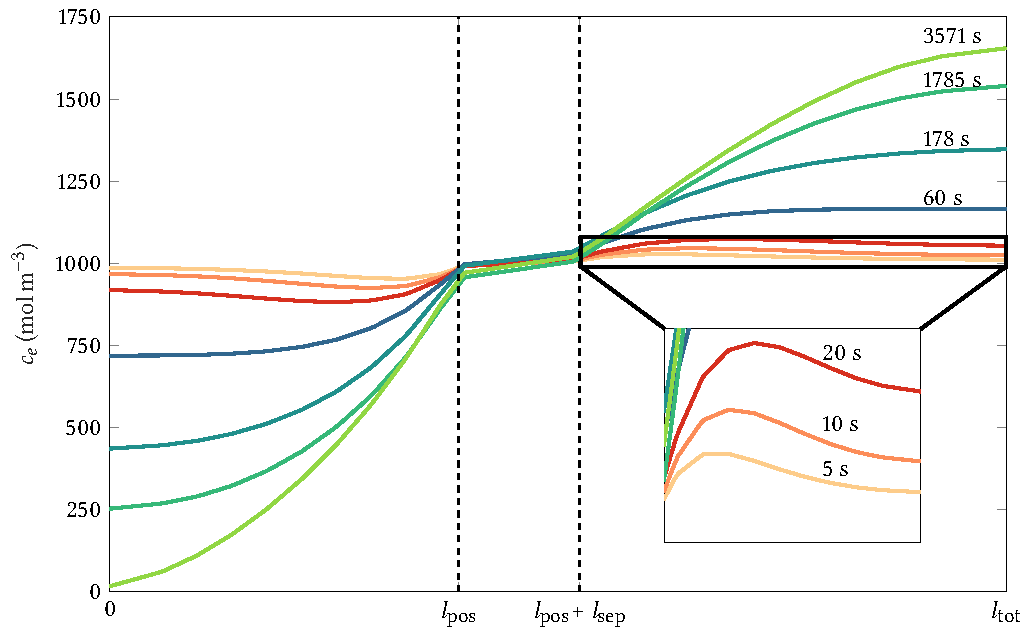
\includegraphics{ce_1C_at_various_times.pdf}
    \caption[Electrolyte conc.\ (time-snapshots) along cell thickness for 1C~discharge]{\ch{Li^+} ion concentration in electrolyte along cell thickness
        at various time-snapshots during a 1C~discharge simulation of the
        \glsfmtshort{p2d} model. A \glsfmtlong{qss} (\glsfmtshort{qss}) spatial
        profile  with inflection point at each separator interface begins to
        form at \approx \SI{60}{\second} after discharge begins. However, the
        ionic concentration in electrolyte exhibits a significantly different
        transient behaviour (zoomed inset) possessing another inflection point
        that disrupts the monotonic trend. Depletion of ionic concentration at
        positive current collector  towards end of discharge is also seen
    (bottom left).}
    \label{fig:ce1cdischgwithzoom}
\end{figure}

Although  not presented  in the  context  of incorporating  into the  \gls{spm},
Guduru~\etal~\cite{Guduru2012}   derived   an   analytical   solution   of   the
spatio-temporal  evolution  of  electrolyte concentration  using  the  \gls{sov}
method. The \gls{sov} method was first  applied to lithium ion cell modelling by
Subramanian~\etal~\cite{Subramanian2001a}  in order  to  solve  for solid  phase
concentration  profiles in  spherical  electrode particles.  Although the  ionic
concentration  in  the electrolyte  computed  by  the analytical  expression  in
Guduru~\etal{} seems like a feasible choice for inclusion into the \gls{spm}, it
is only applicable for galvanostatic  boundary conditions \ie~when the applied
current  is held  constant over  time. By  natural extension,  researchers could
hypothesise  that this  restriction  may  be removed  by  considering the  input
current as  piecewise constant  over small sample  intervals. Such  a hypothesis
could  be  reinforced  by  the  fact that  standard  drivecycles  are  specified
as  discrete  samples and  the  discrete-time  \gls{spm} processes  these  input
samples assuming \gls{zoh} behaviour. However, the analytical solution presented
in  Guduru~\etal{}  assumes  a  \gls{qss} concentration  profile.  The  authors'
presentation  considers a  near-instantaneous  establishment  of this  \gls{qss}
and  suggests a  parameter  independent analysis  through  use of  dimensionless
concentrations and time-constants instead of absolute time.

In  the  studies  conducted  by  this  thesis  author,  significantly  different
transient  behaviour  is exhibited  by  the  electrolyte concentration  profile.
Furthermore,  the  time  taken  to   establish  the  \gls{qss}  profile  is  not
negligible. This  difference in behaviour  could be attributed to  the different
parameter  set used.  \Cref{fig:ce1cdischgwithzoom}  shows  the spatial  profile
of  ionic concentration  at  various  snapshots of  time  during  a 1C~constant
current  discharge.  Starting  at \SI{100}{\percent}  \gls{soc},  the  discharge
lasts  \SI{3571}{\second}. It  is  seen that  it  takes nearly  \SI{60}{\second}
to  establish  the approximately  parabolic  shape  assumed by  the  electrolyte
concentration. After the initial transient has elapsed, the underlying structure
of the mathematical equations can be assumed  to be static. This is evidenced by
the  fact that  at  \SI{1785}{\second} \ie~after half  of  the discharge  is
completed, the shape of the curve is  nearly identical to the one towards end of
discharge. These  \gls{qss} curves  have their sole  inflection points  at their
separator  interfaces and  remains monotonic  within their  respective electrode
regions.  The  difference in  height  for  various  times  can be  accounted  by
the  coefficients  solved  using  the  analytical  modal  solution  proposed  in
Guduru~\etal{}.

The  axes  in  the  inset  of \cref{fig:ce1cdischgwithzoom}  shows  a  zoomed-in
view  of  the electrolyte  concentration  during  the transient  phase,  wherein
the  \gls{qss}  has  not  yet  been  established.  In  particular,  there  exist
additional inflection points,  one within the interior of  each electrode, which
renders the transient concentration profile mathematically incompatible with the
monotonicity  exhibited  by  the  \gls{qss} profile.  Thus,  in  highly  dynamic
operating  conditions with  frequent reversals  in  the direct  of current,  the
\gls{qss} assumption for the galvanostatic analytical solution becomes harder to
uphold without introducing significant  errors. Finally, the analytical solution
profile in Guduru~\etal{}  is not amenable to embedded  implementation, since it
consists of a non-trivial set of trigonometric computations at each time-step.

Prada~\etal~\cite{Prada2012} were  the first to provide  a simplified expression
for potential drop in the electrolyte  by including the terms representing ionic
concentration gradient within the cell thickness. Thus, \cref{eq:electrolytepd}
gets modified as
\begin{equation}\label{eq:electrolytepdwithce}
    \phi_\epos - \phi_\eneg = (1-t_{+}^0) \frac{2RT}{F}\ln \frac{c_\text{e,\tiny pos/cc}}{c_\text{e,\tiny neg/cc}}-\frac{I}{2 A}\left(\frac{l_\text{neg}}{\kappa_\text{eff,neg}} + 2 \frac{l_\text{sep}}{\kappa_\text{eff,sep}} + \frac{l_\text{pos}}{\kappa_\text{eff,pos}}\right)
\end{equation}
Although  the complete  expression for  electrolyte overpotential  was provided,
it   was  presented   in  a   cursory  manner \ie~without   detailing  the
spatio-temporal  computation  of  ionic  concentration  values  at  the  current
collector interfaces. Nevertheless, it is important to note this contribution as
\cref{eq:electrolytepdwithce} is widely relied upon by subsequent literature and
shall be used in \cref{sec:newelectrolytemodel}.

% in the original work of electrolyte concentration distributio presented by thisn
% thesis author i                                                                n


Rahimian~\etal{}~\cite{KhaleghiRahimian2013}   were   the   first   to   provide
approximate expressions for both charge  transport and mass transport properties
of the electrolyte specifically with the focus on improving the basic \gls{spm}.
The  authors discuss  the usage  of a  polynomial approximation  for electrolyte
concentration and potentials.  In particular, a cubic polynomial  was chosen for
approximating the  electrolyte concentration within the  porous electrodes. This
necessitates the  need to solve  for eight coefficients for  uniquely describing
the electrolyte concentration profile within  the electrode regions. However, in
the standard \gls{dfn} model, the number of electrolyte-specific \glspl{pde} and
their corresponding boundary conditions describing  charge and mass transport is
insufficient to uniquely  solve for all unknown coefficients  of this polynomial
approximation.  A detailed  explanation  of this  equation  deficiency shall  be
discussed in \cref{subsec:quadraticsimresultsanalysis}.

To overcome the issue of  equation deficiency, Rahimian~\etal{} adopted a scheme
wherein one  additional spatial location in  the interior of each  electrode was
also needed. The coefficients of the polynomial approximation were then obtained
by iteratively solving a large  coupled system of algebraic equations, embedding
within  them  the additional  equations  evaluated  at  the interior  points.  A
complicating issue  that arises  is regarding the  optimal positioning  of these
additional interior  points. An online  numerical optimisation was  performed to
obtain  the optimal  placement of  this interior  node. In  the opinion  of this
thesis author, these optimisation results could be sensitive to the thickness of
the electrodes  among other  parameters. A  discussion of  the stability  of the
proposed routine and its robustness to  parameter variance shall help in lending
confidence in the proposed method.  Although sufficient accuracy of the improved
\gls{spm} was  demonstrated for  currents up  to 5C, a  notable omission  is the
discussion of the model's performance  to dynamic input profiles. In conclusion,
the author of this thesis opines that, although this method serves as a proof of
concept towards implementing polynomial approximations for electrolyte dynamics,
until the aforementioned  gaps are addressed with clarity, it  is not convincing
for uptake by relevant stakeholders.

Kemper  and  Kum~\cite{Kemper2013} presented  an  approach  wherein the  spatial
gradients  of the  electrolyte concentration  are neglected.  The time-evolution
of  \emph{average}  ionic  concentration  in  each of  the  three  cell  regions
\viz~positive electrode,  separator and  negative electrode  are described  by a
set  of three  \glspl{ode}.  As  established by  the  discussion  thus far,  the
concentration gradients  along the axial  thickness of the cell  is significant,
even at  moderate {C-rates}.  Lending strength  to doubts  on the  model's wider
applicability  is the  fact that  results  from constant  current inputs  (which
induce large concentration  gradients in electrolyte) have not  been reported in
this work. Thus,  this approach is deemed as not  satisfactory enough to warrant
further engagement.

Luo~\etal~\cite{Luo2013} derived  a parabolic  approximation of  the electrolyte
concentration  distribution along  the  thickness of  the  cell. The  derivation
is  obtained  for  the case  of  steady-state  wherein  the  rate of  change  of
concentration  is  zero.  However,  the  author  of  this  thesis  is  sceptical
about  this since  in  the simulations  performed there  is  no situation  other
than  prior to  application of  current that  this exact  steady-state condition
is  satisfied.  In  the  \gls{qss}   profile  concept  discussion  based  on  on
\cref{fig:ce1cdischgwithzoom}, it is clear  that only the \emph{spatial} profile
reaches a shape that can be  potentially described by a mathematically invariant
family of curves. The electrolyte concentration is still \emph{time-varying} and
therefore violates the static time-evolution assumption. Although Luo~\etal{} do
not explicitly acknowledge this, they provide an extension for general operating
conditions  by introducing  exponential scaling  functions~$f_n(t)$ and~$f_p(t)$
while retaining the  assumption of parabolic spatial  behaviour. The computation
of certain time-constants in these scaling functions are not elucidated nor is a
summary  of procedural  steps for  determination of  the aforementioned  scaling
functions provided.


In a subsequent paper by  the same authors \ie~Luo~\etal~\cite{Luo2013a}, the
electrolyte concentration  model together  with a  similarly-derived electrolyte
potential model  was incorporated into  the conventional \gls{spm} to  arrive at
what the authors term as extended \gls{spm}. In this work, the electrolyte
potential is set to account for contribution from two terms ---
\begin{enumerate*}[label=\emph{\alph*})]
    \item ohmic drop due to bulk solution resistance and
    \item polarization potential due to concentration gradients
\end{enumerate*}
Although it  seeks to correctly account  for the two causes  of overpotential in
the  electrolyte,  there  is  no  detailed explanation  on  the  computation  of
quantities such as time-constants involved in the polarization potential term.

A modified version of the electrolyte model proposed in Luo~\etal~\cite{Luo2013}
was  used  in Zou~\etal~\cite{Zou2016a}  for  observer  design in  an  \gls{soc}
estimation  application. The  modification  essentially  consists of  truncating
the complex  expression in~\cite{Luo2013}  consisting of  six coefficients~$p_1$
through~$p_6$ to just two, and elimination of the aforementioned time-constants.
However, to  the disappointment  of the  author of this  thesis, the  claim that
truncation to~$n=2$ terms is sufficient to  describe the dynamics proved  to be
optimistic for  the parameter set considered.  In my attempts to  reproduce this
work, an  arbitrary scaling  factor was  needed to  correct for  the electrolyte
potential drop  and match  the \gls{p2d} simulations.  The requirement  for such
scaling factors  whose physical  origins are not  clearly identifiable  lends to
scepticism on the model's robustness. Furthermore,  it was found that this value
needed to be  hand-tuned for each parameter-set. Until these  gaps are addressed
clearly, it is worth seeking other  viable alternatives to model the electrolyte
dynamics.

After  completing  the  simulations  with  the  aforementioned  scaling  factors
and  continuing  in  the  quest  for other  alternatives,  the  author  of  this
thesis  made  an observation  that  other  researchers  have  had to  resort  to
similar techniques  for describing the electrolyte  overpotential. For instance,
Han~\etal~\cite{Han2015a}  use a  similar  scaling factor~$p<0$  for the  entire
expression   of  \cref{eq:electrolytepdwithce}   representing  the   electrolyte
overpotential   using  the   polynomial  approximation   approach  proposed   by
Rahimian~\etal~\cite{KhaleghiRahimian2013}.  However, these  unexplained scaling
factors lower the confidence regarding the model's general applicability.


Tanim~\etal~\cite{Tanim2014}  accounted  for  electrolyte dynamics  by  deriving
reduced   order  transfer   functions  for   ionic  concentration   distribution
and   electrolyte  overpotential   using  the   \gls{ima}  technique.   However,
the  coefficients  of   these  transfer  functions  are   excessively  long  and
comprised  of   chained  algebraic   operations  expressed  in   a  high-entropy
sum-of-products  form  in  the  appendix   of  their  work.  For  instance,  ten
coefficients  are  needed  to  describe  the  concentration  profile  while  six
coefficients  are required  for  the electrolyte  potential.  The median  length
of  each  atomic  sub-expression  of these  coefficients  is  sufficiently  high
to  obfuscate   their  physical  significance.   A  low-entropy  form   for  the
coefficients  of  these   transfer  functions  similar  to   that  pioneered  by
Middlebrook~\cite{Middlebrook} and  exemplified in the  design-oriented analysis
of  electric   circuits~\cite{Middlebrook1998,Vorperian2002}  could   have  been
helpful to aid the readers' understanding.  The author of this thesis recognises
that  mathematical complexity  should  not be  the sole  basis  to evaluate  the
merits of  such proposed improvements.  Although the presentation of  these long
coefficients have been judiciously moved  to the appendix, their derivations ---
essential to prove the model's validity  --- is curiously omitted. The length of
the mathematical  expressions increases  the probabilities of  introducing human
errors during implementation.

It  is worth  noting that  Marcicki~\etal~\cite{Marcicki2013} had  independently
proposed a similar approach \viz~deriving a transcendental transfer function
from  electrolyte  concentration  to  applied  current, albeit  for  a  cell  of
\gls{lfp} chemistry. This transfer function  consisted of a series of hyperbolic
trigonometric functions which  were later truncated by  Padé approximation (see
\cref{subsec:freqdomainroms}  for  a  brief  introduction  to  frequency  domain
\glspl{rom}). However, upon trying this approach for the \gls{lco} parameter set
by this thesis'  author, in order to obtain sufficient  accuracy, the truncation
order had  to be  raised to  at least seven,  similar in  complexity to  that of
Tanim~\etal~\cite{Tanim2014a}.  In  both Marcicki~\etal~\cite{Marcicki2013}  and
Tanim~\etal~\cite{Tanim2014a},  the  electrolyte-specific  enhancements  to  the
\gls{spm} are in  the frequency domain, placing further  burden, particularly on
industry stakeholders to accurately interpret  and transform the coefficients to
a time-domain implementation  for deployment in an embedded  \gls{bms}. Owing to
this,  as  already  stated in \cref{subsec:freqdomainroms},  these  models  fall
outside the scope of this thesis.
% ignoring prof plett's latest work on electrolyte transfer functions

Fan~\etal~\cite{Fan2016}   proposed   an   Extended  \gls{spm}   that   includes
electrolyte dynamics using  the \gls{gpm} which achieves  an acceptable accuracy
in terminal voltage  performance. Although the authors claim  that the \gls{spm}
is computationally  \emph{cheaper} than  other model order  reduction techniques
such as proper orthogonal decomposition  and balanced truncation, this claim has
not  been substantiated.  The sole  comparison of  CPU times  presented in  this
work  only compares  against  the classical  \gls{fdm}.  Although an  impressive
computational  speed is  achieved, it  is unclear  whether the  model equations,
particularly  those  involving  solutions  of  non-linear  integral  expressions
resulting from  applying the Galerkin's  method can  be solved in  real-time for
embedded implementation.  In the review of  this method conducted by  the author
of  this thesis,  it  appears  that the  Galerkin's  projection  method is  more
suitable  for  desktop  simulations.  In  congruence  with  my  scepticism,  the
authors  of~\cite{Fan2016} have  not claimed  the suitability  of this  work for
online/embedded  application  in a  \gls{bms}.  Therefore,  as per  this  thesis
authors' stance  explained in \cref{sec:classificationscheme},  models employing
such methods are deemed to be not in alignment with the goals of this thesis.

Moura~\etal~\cite{Moura2017} proposed an improved \gls{spm} by simply augmenting
the  conventional  \gls{spm}  with  a simplified  form  of  electrolyte-specific
equations of  the original  \gls{dfn} model. The  resulting model  therefore has
\glspl{pde} in it and therefore not easily amenable for embedded implementation.
Lotfi~\etal~\cite{Lotfi2017}  presented  an   algebraic  approximation  for  the
spatial  distribution   of  electrolyte  concentration  by   modifying  standard
parabolic expressions with leading exponential  coefficients. There are two main
issues with this approach. It is not explained why this mathematical formulation
was chosen  and its superiority  with respect to other  family of curves  is not
discussed. Secondly, these coefficients are to be determined through solution of
equations obtained by applying continuity  and flux boundary conditions from the
\gls{dfn}  model  for  electrolyte  concentrations  at  the  electrode-separator
interfaces. Since exponential-type expressions are assumed, the resulting set of
equations are non-linear,  the solving of which, especially in  the context of a
resource-constrained environment is problematic.

% The other main contribution of this work is its feasibility analysis of having
% convergent  estimators for  this model  and design  of such  a \gls{pde}-based
% estimator.  In  the  views of  this  thesis  author,  this  approach is  on  a
% trajectory that deviates  too far from a simplified model  suitable for online
% implementation.

In  the  authors'   observations  in  trying  to  replicate   the  results  from
the  literature  presented here,  the  errors  in  all such  approximations  can
be  attributed  to  inaccuracies  in  computing  the  spatio-temporal  evolution
of  electrolyte   concentration.  Upon   obtaining  a   good  estimate   of  the
electrolyte concentration profile, \cref{eq:electrolytepdwithce} is deemed to be
satisfactory for  the electrolyte  overpotential computation. Thus  attention is
focussed on solving for the electrolyte concentration profile.

From the discussion of literature, it is clear that the proposed enhancements to
the  computing the  ionic concentration  in electrolyte  falls into  one of  the
following two categories
\begin{itemize}
    \item model description through physical principles followed by mathematical
        simplification
    \item fitting of pre-assumed simplified mathematical structures to some
        physical phenomena
\end{itemize}

In the  views of the  author, it appears that  using the former  approach yields
technically  correct, yet  mathematically convoluted  expressions overpotentials
that are fraught with implementation  difficulties. Although the latter approach
looks  promising  in   terms  of  ease  of   implementation,  their  sub-optimal
performance and lack of wider-applicability leaves much to be desired. Among the
latter  class of  models, owing  to  its simplicity,  the quadratic  (parabolic)
approximation method for  electrolyte concentration is an  attractive option. It
is therefore  important to understand  the source  of weakness of  this specific
sub-class of  models. Such  an analysis  has not  been performed  in literature.
Hence,  the  author's  analysis  on   the  quadratic  approximation  method  for
electrolyte concentration is presented next in \cref{sec:quadraticapprox}.


% May also mention some typographical errors in Lotfi etal second paper
% Mention that parabolic profile is a common theme
% perhaps it cannot be done, but we do not give up. Equation deficiency

% But I  did something different. The high accuracy  of the \gls{soc}
% in  the  basic  \gls{spm}  leads  to  the  author's  hypothesis  that  if  the
% electrolyte  concentration  can be  solved  as  an independent  subsystem  and
% incorporated into the terminal voltage, this can lead to an improved \gls{spm}
% with electrolyte  dynamics. Such  a decoupled  electrolyte inclusion  into the
% basic \gls{spm}\fxnote{fix this sentence}

